%----------------------------------------------------------------------------------------
%	CONFIGURATIONS
%----------------------------------------------------------------------------------------

\documentclass[10pt,a4paper,oneside]{article}

\usepackage[utf8]{inputenc}
\usepackage{graphicx}
\usepackage{epstopdf}
\usepackage{natbib}
\usepackage{amsmath}
\usepackage{multirow}
\usepackage{lipsum}
\usepackage{caption}
\usepackage{subcaption}
\usepackage[a4paper,left=2cm,right=2cm,top=2.5cm,bottom=2.5cm]{geometry}

%----------------------------------------------------------------------------------------
%	INFORMATION
%----------------------------------------------------------------------------------------

\title{Estudo de paralelismo num problema de simulação discreta}

\author{Filipe Figueiredo\footnote{Filipe Figueiredo - 201203559},
  Pedro Paredes\footnote{Pedro Paredes - 201205725}, DCC - FCUP}

\date{Dezembro 2015}

\renewcommand{\tablename}{Tabela}
\renewcommand{\figurename}{Figura}
\renewcommand{\refname}{Referências}
\newcommand{\BigO}[1]{\mathcal{O}(#1)}

\makeatletter
\makeatother

\begin{document}

\maketitle

%----------------------------------------------------------------------------------------
%	SECTION 1
%----------------------------------------------------------------------------------------

\section{Introdução}
\label{sec:intro}
Neste trabalho discutimos um problema de simulação de eventos
discretos determinística numa grelha e exploramos diferentes
estratégias de paralelismo possíveis.

Este tipo de problemas é notoriamente difícil de se paralelizar devido
às dependências existentes nos dados e na topologia da simulação
provenientes das restrições impostas pelo problema. Neste trabalho, a
topologia da simulação é regular (uma grelha retangular) o que permite
que abordagens simples sejam efetivas, mas no geral é necessário
recorrer a métodos mais complexos como computação especulativa.

Focamo-nos em três abordagem simples, que aproveitam diferentes
aspetos do problema. Além disso, exploramos diferentes esquemas de
redistribuição de trabalho de modo a podermos manter eficiência em
\textit{inputs} desbalanceados.

O resto deste relatório será organizado da seguinte forma. Na
Secção~\ref{sec:prob} descrevemos o problema com algum pormenor e as
dificuldades em o paralelizar. Na Secção~\ref{sec:par} introduzimos as
estratégias para paralelizar o problema e fazemos uma comparação
teórica entre elas. Na Secção~\ref{sec:res} apresentamos os resultados
experimentais obtidos pela implementação de cada estratégia referida
na secção anterior. Finalmente, na Secção~\ref{sec:con} fazemos
algumas notas finais.

%----------------------------------------------------------------------------------------
%	SECTION 2
%----------------------------------------------------------------------------------------

\section{Descrição do problema}
\label{sec:prob}
O problema que pretendemos estudar é uma simulação numa grelha
retangular de $R$ linhas por $C$ colunas. Cada célula da grelha pode
estar vazia ou conter um dos seguintes elementos: uma pedra, um coelho
ou uma raposa. A simulação é feita iterativamente, ou seja, a partir
de uma geração inicial (o \textit{input}), representada por uma
distribuição de pedras, coelhos e raposas numa grelha, é gerada uma
nova geração seguindo um conjunto de regras fechado e o mesmo é
repetido $N_G$ vezes até se obter a geração final (o
\textit{output}). Representamos por $N_i$ o número de coelhos e
raposas existentes na geração $i$.

As regras de construção de uma nova geração começam por primeiro mover
todos os coelhos simultaneamente para uma nova célula que esteja
vazia, seguindo uma ordem determinística. Seguidamente as raposas são
movidas para uma célula vazia ou para uma célula que contenha um
coelho. O último caso representa uma raposa a comer um coelho, o que
na prática significa que o coelho que foi comido desaparece da
simulação na nova geração. Adicionalmente, tanto os coelhos como as
raposas podem procriar, duplicando-se cada animal num período
regular. A Figura~\ref{fig:sim} exemplifica duas gerações de uma
simulação.

\begin{figure}
    \centering
    \begin{subfigure}[b]{0.3\textwidth}
        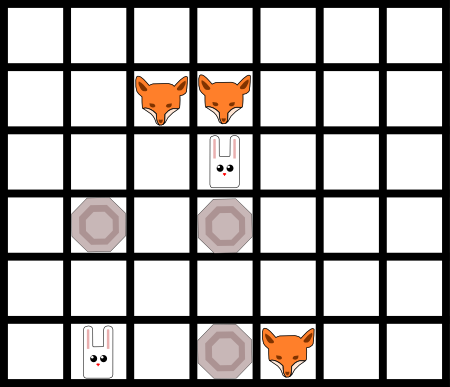
\includegraphics[width=\textwidth]{grid1.png}
        \caption{Geração 1}
    \end{subfigure}
    ~
    \begin{subfigure}[b]{0.3\textwidth}
      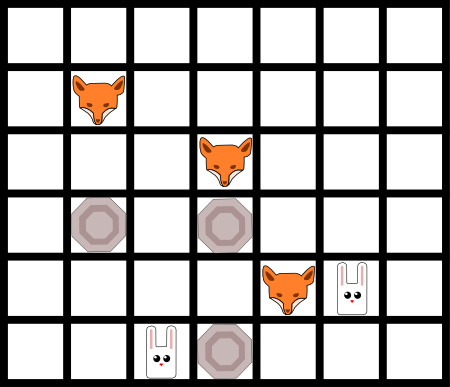
\includegraphics[width=\textwidth]{grid2.png}
      \caption{Geração 2}
    \end{subfigure}
    \caption{Exemplo de duas gerações de uma simulação}
    \label{fig:sim}
\end{figure}

A partir desta descrição simples do problema é possível identificar
dependências fortes do problema. Em cada nova geração, a simulação das
raposas só pode ser iniciada após a conclusão da simulação de todos os
coelhos, pois os movimentos dos coelhos condicionam os movimentos das
raposas (a dependência é apenas local, ou seja, um coelho muito
afastado de uma certa raposa não condiciona o seu movimento, mas
aproveitar este tipo de observações requer um algoritmo mais complexo
e menos óbvio de paralelizar e não foi por isso considerado). Assim,
existe aqui um ponto de sincronização necessário na execução da
simulação.

Adicionalmente, a simulação dos coelhos também impõe certas restrições
nos movimentos dos coelhos entre si. Além de serem obstáculos uns para
os outros, podem existir conflitos no movimento de dois ou mais
coelhos que se podem movimentar para a mesma célula. Nesse caso apenas
um coelho sobrevive e por isso é necessário sincronizar os coelhos que
após a resolução de conflitos se mantêm. Isto é análogo para as
raposas.

É de notar que este tipo de simulação tem uma natureza exponencial
associada. Apesar de ser possível limitar o crescimento dos coelhos e
raposas atribuindo-lhes valores altos para o período para procriação,
as simulações mais ``interessantes'' (leia-se mais movimentadas)
rapidamente (em poucas gerações) preenchem a grelha a mais de
$50\%$. Por esta razão, não consideramos representações esparsas da
grelha (isto é, que não guardam a grelha diretamente como uma matriz),
pois além de serem menos eficientes têm aplicabilidade reduzida.

%----------------------------------------------------------------------------------------
%	SECTION 3
%----------------------------------------------------------------------------------------

\section{Estratégias de paralelização}
\label{sec:par}


%----------------------------------------------------------------------------------------
%	SECTION 4
%----------------------------------------------------------------------------------------

\section{Resultados e discussão}
\label{sec:res}


%----------------------------------------------------------------------------------------
%	SECTION 5
%----------------------------------------------------------------------------------------

\section{Conclusão e notas finais}
\label{sec:con}

%\bibliographystyle{plain}
%\bibliography{report}

\end{document}
